\documentclass[12pt]{article}
\usepackage[utf8]{inputenc}
\usepackage[russian]{babel}
\usepackage{mathrsfs}
\usepackage{amssymb}
\usepackage{amsmath}
\usepackage{graphicx}
\usepackage{bbm} % для индикатора
\usepackage{chngcntr} % без этого пакета у меня не робит counterwithin
\usepackage{ulem} % нужен для \uline, которая умеет переносить подчеркнутый текст
\usepackage{tikz}  
\usepackage{pb-diagram}
\usepackage{pgfplots}
\usepackage{caption}
\usetikzlibrary{arrows,decorations.pathmorphing,backgrounds,positioning,fit,petri}
\usepgflibrary{arrows.meta}
\usetikzlibrary{arrows.meta}

\graphicspath{{pictures/}}
\DeclareGraphicsExtensions{.pdf,.png,.jpg}

\textheight=24cm
\textwidth=16cm
\oddsidemargin=0pt
\topmargin=-1.5cm
\parindent=24pt
\parskip=0pt
\tolerance=2000
\flushbottom

\newtheorem{Th}{Теорема}
\newtheorem{Def}{Определение}
\newtheorem{Lem}{Лемма}
\newtheorem{St}{Утверждение}

\newenvironment{Proof}{\par\noindent{\bf Доказательство}}{$\blacksquare$} 
\newenvironment{Ex}{{\bf Пример}\ }{}
\newenvironment{Wtf}{
\includegraphics[height=5mm]{ping}}{}
\newenvironment{Why}{
\includegraphics[height= 5mm]{cat}}{}

\numberwithin{Th}{section}
\numberwithin{Def}{section}
\numberwithin{Lem}{section}
\numberwithin{St}{section}
\numberwithin{equation}{section}
\counterwithin*{section}{part}

\newcommand\Set[2]{\left\{ #1 \colon #2 \right\}}
\newcommand\Pro{\mathbb{P}} % вероятность
\newcommand\Ev{\mathscr{A}} % алгебра событий
\newcommand\Bor{\mathscr{B}} % борелевская сигма-алгебра
\newcommand\Real{\mathbb{R}} % вещественная прямая
\newcommand\Expec{\mathbb{E}} % матожидание 
\newcommand\Disp{\mathbb{D}}  % дисперсия
\newcommand\Ind{\mathbbm{1}} % индикатор
\newcommand\Med{{\rm med \,}} % медиана
\newcommand\xequiv[1]{\stackrel{\mathrm{ #1}}{\equiv}}


\begin{document}

\tableofcontents
\newpage

\part{Теория вероятности}

\textit{Ты спросишь меня, кого я люблю больше: тебя или теорию вероятности. Я отвечу, что почти наверное тебя и ты уйдешь, так и не узнав, что почти наверное значит с вероятностью 1.}

\newpage

\section{Вероятностное пространство}
\qquad Методы теории вероятности работают в ситуациях, называемых стохастическими. Для них характерны три свойства:
\begin{enumerate}
	\item Непредсказуемость 
	\item Воспроизводимость 
	\item Устойчивость частот
\end{enumerate}

Для описания стохастических ситуаций ситуаций необходимо определить функцию вероятности. Её область определения назывется множеством событий.
В свою очередь событие (такое как, например, выпадание чётного числа на кубике) могут являться совокупностью неких более простых событий, описывающих стохастическую ситуацию (число, выпавшее на кубике). Последнее множество называется множетсвом элементарных исходов и обозначается $\Omega$.  

Множество событий, обозначаемое $\Ev$, должно обладать следующими интуитивными свойствами:
\begin{enumerate}
	\item Отрицание события есть событие (если <<пойдет дождь>> событие, то <<не пойдет дождь>> также событие)
	\item Объединение событий есть событие (<<пойдет дождь>> или <<пойдет снег>>)
	\item Все множество элементарных исходов является событие (<<Что-нибудь да произойдет>>)
\end{enumerate}

Формализуя эти свойства, получаем определение алгебры.
\begin{Def}
Семейство $\Ev$ подмножеств множества $\Omega$  называется \\ \underline{алгеброй}, если 
\begin{enumerate}
	\item $\forall A \in \Ev, B\in \Ev \Rightarrow A \bigcup B \in \Ev$
	\item $\forall A \in \Ev \Rightarrow \overline{A} \in \Ev$
	\item $\Omega \in \Ev$
\end{enumerate}
\end{Def}

Из аксиом алгебры и формулы $A\bigcap B = \overline{\overline{A} \bigcup \overline {B}}$ следует, что пересечений событий явялется событием.

Наименьшей возможной алгеброй является $\left\{ \Omega, \varnothing \right\}$

\begin{Def}
Семейство $\Ev$ подмножеств множества $\Omega$  называется \\ \underline{$\sigma$-алгеброй}, если 
\begin{enumerate}
	\item $\forall A_1, \dots, A_n, \ldots \in \Ev \Rightarrow \bigcup\limits_{i=1}^{\infty} A_i \in \Ev$
	\item $\forall A \in \Ev \Rightarrow \overline{A} \in \Ev$
	\item $\Omega \in \Ev$
\end{enumerate}
\end{Def}

\begin{Def}
Пусть $\mathscr{K}$ - класс подмножеств $\Omega$. $\sigma$-алгебра $\sigma (\mathscr{K})$,\\ \underline{ порожденная классом $\mathscr{K}$} --- наименьшая $\sigma$-алгебра, 
содержащая $\mathscr{K}$, то есть любая $\sigma$-алгебра, содержащая $\mathscr{K}$, содержит и $\sigma (\mathscr{K})$.
\end{Def}
\begin{Ex}
$\sigma$-алгеброй, порожденной $\mathscr{K} = A$, будет являться $\sigma(A) = \left\{ \varnothing, A, \overline(A), \Omega \right\}$.
\end{Ex}

$\sigma$-алгебра является более узким понятием, нежели алгебра, то есть любая $\sigma$-алгебра является алгеброй, а обратное, вообще говоря, неверно. \\
\begin{Ex}
Пусть $\Omega = \mathbb{R},\  \Ev$ содержит конечные подмножества $\Omega$ и их дополнения. Для такого множества выполнены все аксиомы алгебры: 
$\Omega = \overline{\varnothing} \in \Ev$, объединение конечных множеств есть конечное множество, объединение конечного множества с дополнением к конечному 
множеству так же является дополнением к некоторому множеству. То же можно сказать и об объединении двух дополнений. Таким образом, $\Ev$ является алгеброй.
Все элементы $\Ev$ либо конечны, либо континуальны, поэтому $\Ev$ не содержит $\mathbb{N}$. Но $\mathbb{N} = \bigcup\limits_{i=1}^{\infty}\{i\}$, то есть
не выполнено свойство счетной аддитивности из определения $\sigma$-алгебры.
\end{Ex}

\begin{Def}
Пара $(\Omega, \Ev)$ называется \underline{измеримым пространством}, если $\Ev$ является $\sigma$-алгеброй. Если же $\Ev$ - алгебра, то  $(\Omega, \Ev)$ --- \underline{измеримое пространство} \underline{ в широком смысле}.
\end{Def}

\begin{Def}
\underline{Вероятностью} называется функция $\Pro \colon \Ev\rightarrow \mathscr{R}_+$, удовлетворяющая свойстам
\begin{enumerate}
	\item $\forall A \in \Ev \quad \Pro (A) \ge 0$
	\item $\forall A_1, \dots, A_n, \ldots \in \Ev \quad A_i \bigcap A_j  = \varnothing\  (i \not= j)  \Rightarrow \Pro (\bigcup\limits_{i=1}^{\infty} A_i) = \sum\limits_{i = 1}^{\infty} A_i$
	\item $\Pro (\Omega) = 1$
\end{enumerate}
\end{Def}

\begin{Def}
\underline{Вероятностным пространством} $(\Omega, \Ev, \Pro)$ называется измеримое пространство $(\Omega, \Ev)$, снабженное вероятностью $\Pro$.
\end{Def}
\begin{Wtf}
Кому вообще нужна $\sigma$-алгебра событий, и зачем весь этот огород, если можно рассматривать множество всех подмножеств множества $\Omega$? Когда-то кто-то доказал, что в случае очень большого множества элементарных исходов, например, континуального, множество $2^{\Omega}$ будет иметь такую крокодильски большую мощность, что вся теория сломается. Таким образом, алгебры нужны для того, чтобы вероятность имела хорошую область определения.
\end{Wtf}

\paragraph{Свойства вероятности}
\begin{enumerate}
	\item $\Pro (\varnothing) = 0$ 
	\item $\Pro (\overline{A}) = 1 - \Pro (A)$
	\item $A \subseteq B \quad \Rightarrow \Pro (A) \le \Pro (B)$
	\item $\Pro (A) \le 1$
	\item $\Pro (A \bigcup B) = \Pro (A) + \Pro (B) - \Pro (AB)$ 
	\item $\Pro (A \bigcup B) \le \Pro (A) + \Pro (B)$ 
	\item $\Pro (\bigcup\limits_{i=1}^{n} A_i) = \sum\limits_{k=1}^{n} \sum\limits_{i_1<\dots <i_k} (-1)^{k+1} \Pro(A_{i_1}A_{i_2}\ldots A_{i_k})$
	\item $\Pro (\bigcap\limits_{i=1}^{n} A_i) \ge 1 - \sum\limits_{i=1}^{n} \Pro (\overline{A_i})$ - неравенство Бонферрони
\end{enumerate}

Второй пункт в определении вероятностной меры нельзя заменить аналогичным с конечными объединением и суммой. Однако если добавить к данному требованию так 
называемое свойство непрерывности вероятностной меры, т.е $$\forall B_1, B_2, \ldots \in \Ev \quad B_{n+1} \subseteq B_n \Rightarrow \lim_{n \to \infty} \Pro(B_n) = \Pro(B)$$, то они вместе будут эквивалентны 2. из определения вероятности.

\begin{St}
$\forall A_1, \dots, A_n, \ldots \in \Ev \quad A_i \bigcap A_j  = \varnothing\  (i \not= j)  \Rightarrow \Pro (\bigcup\limits_{i=1}^{\infty} A_i) = \sum\limits_{i = 1}^{\infty} A_i
\Leftrightarrow ( \forall A_1, \dots, A_n \in \Ev \quad A_i \bigcap A_j  = \varnothing\  (i \not= j)  \Rightarrow \Pro (\bigcup\limits_{i=1}^{n} A_i) = \sum\limits_{i = 1}^{n} A_i)  \land  (\forall B_1, B_2, \ldots \in \Ev \quad B_{n+1} \subseteq B_n \Rightarrow \lim\limits_{n \to \infty} \Pro(B_n) = \Pro(B))$
\end{St}
\begin{Proof}
\\ $\Rightarrow$\\
Обозначим $C_n = B_n \setminus B_n+1$. Множества $B, C_1, C_2, \ldots$ не имеют общих точек.\\
$\forall n \quad B_n =  \bigcup\limits_{k=n}^{\infty} C_k \bigcup B$. Тогда $\Pro(B_1) = \Pro(B) + \sum\limits_{k=1}^{\infty} \Pro(C_k)$. Отсюда следует, что ряд в правой части сходится, так как имеет конечную сумму.
$\Pro(B_n) = \Pro(B) + \sum\limits_{k=n}^{\infty} \Pro(C_k)$. При $n \to \infty$ сумма ряда стремится к нулю как остаточный член ряда из предыдущего выражения.
В предельном переходе получаем свойство непрерывности.
\\ $\Leftarrow$\\
Рассмотрим произвольный набор $A_1, A_2, \ldots \in \Ev \quad A_iA_j = \varnothing$.\\
$\Pro(\bigcup\limits_{i=1}^{\infty} A_i) = \Pro(\bigcup\limits_{i=1}^{n} A_i) + \Pro(\bigcup\limits_{i=n + 1}^{\infty} A_i) =\sum\limits_{i = 1}^{n} \Pro(A_i) +  
\Pro(\bigcup\limits_{i=n + 1}^{\infty} A_i) $.\\
 Обозначим $B_n = \bigcup\limits_{i=n + 1}^{\infty} A_i,\quad B_{n+1} \subseteq B_n \quad \forall n,\quad \bigcap\limits_{n=1}^{\infty} B_n= \varnothing$ \\
$\sum\limits_{i=1}^{\infty} \Pro(A_i) = \lim\limits_{n \to \infty} (\Pro(\bigcup\limits_{i=1}^{\infty} A_i) - \Pro(B_n)) = \Pro(\bigcup\limits_{i=1}^{\infty} A_i) - \lim\limits_{n \to \infty} \Pro(B_n) = \Pro(\bigcup\limits_{i=1}^{\infty} A_i)$
\end{Proof}

\begin{Th}[Каратеодори]
Пусть $(\Omega, \Ev)$ --- измеримое пространство в широком смысле, а некоторая функция $\Pro$ обладает свойствами вероятностной меры.Тогда на измеримом пространстве
$(\Omega, \sigma(\Ev))\  \exists !\  \Pro' \colon \forall A \in \Ev \quad \Pro(A) = \Pro'(A)$
\end{Th}
\begin{Proof}
отсутсвует
\end{Proof}\\\\
\begin{Why}
Зачем это нужно? Теорема Каратеодори говорит о том, что любую вероятностную меру, заданную на алгебре, можно однозначно продолжить на $\sigma$-алгебру,
то есть расширить область ее определения. При этом значения функции на алгебре не изменятся. Теорема будет использоваться при определении интеграла Лебега.
\end{Why}
\newpage


\section{Условная вероятность. Независимость событий}

\qquadРассмотрим произвольное $B \in \Ev \colon \quad \Pro(B) > 0$.
\begin{Def}
\underline{Условной вероятностью} события $A \in \Ev$ при условии $B$ называется $\frac{\Pro(AB)}{\Pro(B)} =\colon \Pro(A|B) = \Pro_B(A)$
\end{Def}

Что это означает на пальцах? Условная вероятность $\Pro(A|B)$ --- это веротяность того, что произойдет событие $A$, если мы точно знаем, что произошло событие $B$.\\

\parbox[b][3 cm][t]{20mm}{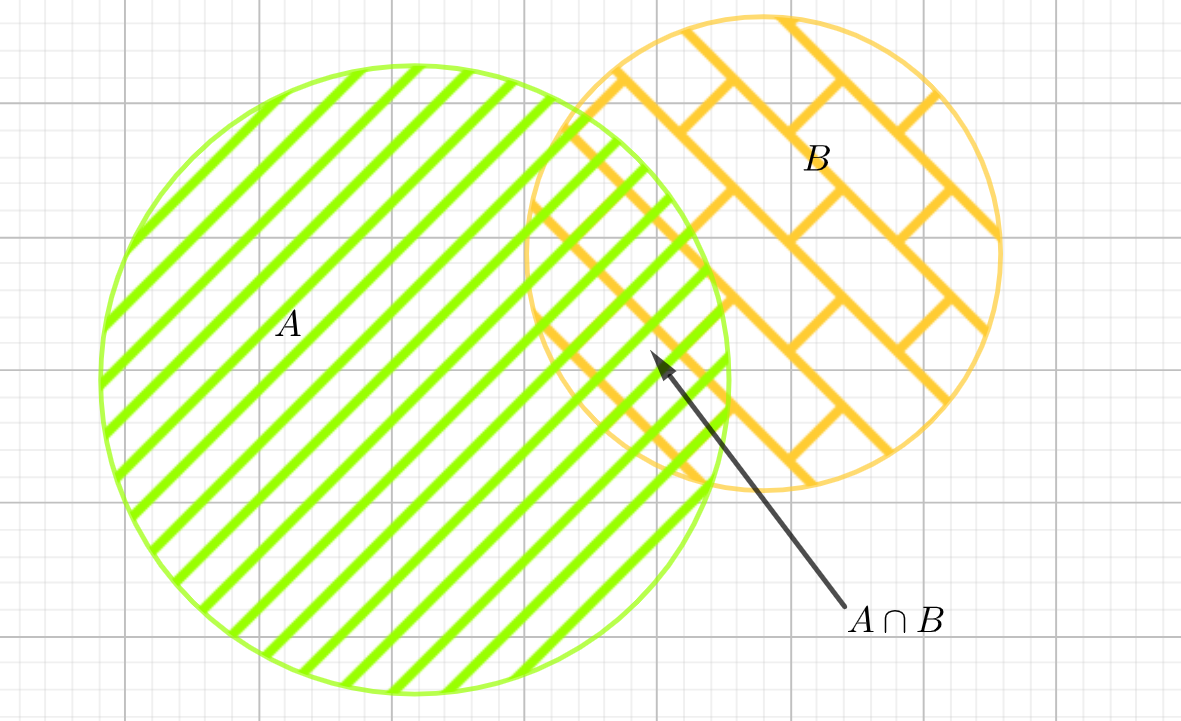
\includegraphics[height=30mm]{cond_prob}}
\hfill
\parbox[b][3 cm][t]{100mm}{
	Графически это означает, что, когда произошло событие $B$, мы оказались в круге $B$. Тогда формула  $\frac{\Pro(AB)}{\Pro(B)}$ есть просто вероятность попасть в $AB$.
}\\

Из определения следует так называемый <<Закон умножения вероятностей>>:
$$\Pro(A|B)\Pro(B)=\Pro(AB)$$

Легко проверяется, что $(B, \Ev_B, \Pro_B)$, где $\Ev_B = \Set{A \bigcap B}{A \in \Ev}$, так же является вероятностным пространством. \\
\begin{Wtf}
Зачем нужно требование $\Pro(B) > 0$, если можно в случае $\Pro(B) = 0$ доопределить условную вероятность нулем как вероятность при условии невозможного события?
При таком доопределении нарушится аксиома 3. вероятности $\Pro_B$, поскольку $\Pro_B(B)$ по доопределению будет равно $0$.
\end{Wtf}

\begin{Def}
События $A, B \in \Ev$ называются \underline{независимыми}, если $$\Pro(AB) = \Pro(A) \Pro(B)$$.
\end{Def}

Для независимых событий $$\Pro(A|B) = \frac{\Pro(A)\Pro(B)}{\Pro(B)} = \Pro(A)$$.\\
\begin{Ex}
Являются ли несовместные события ($AB = \varnothing$) независимыми? Нет, пусть  $A, B \in \Ev \colon \quad \Pro(A) > 0, \ \Pro(B) > 0$. Тогда $\Pro(AB) = \Pro(A)\Pro(B) = 0$, 
что является противоречием. По-простому, если произошло одно из несовместных событий, то второе уже не может произойти, и его условная веротяность равна 0, а не
вероятности самого события, что требуется для независимости.
\end{Ex}

Следующее определение обобщает понятие независимости на произвольное количество событий.
\begin{Def}
События $A_1, A_2, \dots, A_n$ называются \underline{независимыми в совокупности}, если 
$$\forall m = 2, \dots, n \quad \forall 1 \le j_1 < \ldots < j_m \le n \quad 
\Pro(\bigcap_{k=1}^{m}A_{j_k})=\prod_{k=1}^{m} \Pro(A_{j_k})$$
\end{Def}
\begin{Ex}
На примере тетраэдра Бернштейна можно убедиться в том, что попарной независимости событий недостаточно для независимости в совокупности. Рассмотри тетраэдр, у 
которого три стороны покрашены в красный, синий и зеленый, а четвертая содержит все три цвета. События \{выпадет красный\}=\{К\}, \{выпадет синий\}=\{С\}, \{выпадет зеленый\}=\{З\}
попарно независимы (например, вероятность события \{С\}$\bigcap$\{К\} равна веротяности выпадения четвертой грани, т. е. $\frac{1}{4}$, в то время как выпадения 
каждого цвета равна $\frac12$). Однако $\Pro$(\{С\}$\bigcap$ \{К\}$\bigcap$ \{З\}) = $\frac14 \not= (\frac12)^3$.
\end{Ex}
\newpage

\section{Формула полной веротяности. Формула Байеса}

\begin{Def}
$B_1, \ldots, B_n$ образуют \underline{полную группу}, если выполнены следующие условия:
	\begin{enumerate}
		\item $\Pro(B_i) > 0 \quad \forall i = 1, \ldots, n$
		\item $B_iB_j = \varnothing \quad (i \not= j)$
		\item $\bigcup\limits_{i=1}^nB_i = \Omega$
	\end{enumerate}
\end{Def}

\begin{Th}
Пусть $B_1, \ldots, B_n$ образуют полную группу. Вероятность события $A \in \Ev$ можно вычислить по \underline{формуле полной вероятности}:
$$\Pro(A) = \sum\limits_{i=1}^{n} \Pro(A|B_i)\Pro(B_i)$$
\end{Th}

\begin{Proof}
\\
$A=\bigcup\limits_{i=1}^{n}AB_i, \quad AB_i \bigcap AB_j = \varnothing \quad (i \not= j)$ \\
$\Pro(A) = \sum\limits_{i=1}^n \Pro(AB_i) = \sum\limits_{i=1}^{n} \Pro(A|B_i)\Pro(B_i)$ \\
Последний переход следует из  закона умножения вероятностей.
\end{Proof}
\\

Первое требование определения полной группы необходимо для возможности определить условную веротяность, второе позволяет 
разбить множество $A$ на непересекающиеся части. Третье требование, вообще говоря, можно ослабить, потребовав, чтобы $A \subseteq \bigcup\limits_{i=1}^nB_i$.
Доказательство при этом не изменится. \\
\begin{Ex}
Проиллюстрировать формулу полной вероятности можно обычным экзаменом: $A$ - \{студент сдал экзамен\}, $B_i$ - \{студент попал к преподавателю $i$\}.
Как и в любой другой лотерее, можно оценить вероятность попадания к преподавателю $i$, то есть $\Pro(B_i)$, а трезво оценивая свои силы можно прикинуть 
и вероятность сдать тому или иному преподавателю $\Pro(A|B_i)$. Зная все вышеперечисленое, несложно по формуле вычислить вероятность успешной сдачи.
\end{Ex}
\\

Формула полной веротяности используется для вычисления априорной вероятности, т.е. вероятности события, которое  еще не произошло.
Пусть теперь \\$\Pro(A) > 0$. Тогда $\Pro(B_i|A)=\frac{\Pro(AB_i)}{\Pro(A)}$. Используя формулу полной вероятности, получаем \underline{формулу Байеса}:
$$\Pro(B_i|A)=\frac{\Pro(A|B_i)\Pro(B_i)}{\sum\limits_{j=1}^n\Pro(A|B_j)\Pro(B_j)}$$

Формула Байеса используется для вычисления апостериорной вероятности. То есть уже известно, что произошло некоторое событие $A$, и нужно вычислить вероятность
того, что произошло некоторое $B_i$. В примере с экзаменом, например, может быть известно, что студент не сдал экзамен, и хочется вычислить вероятность того, что он
сдавал преподавателю <<Р>>.

\newpage
\section{Случайные величины}

\qquad Случайные события "--- это хорошо, но с события типа <<на монетке выпал герб>> плохо формализуемы, а мы хотим формальности и математичности. Поэтому вместо всяких событий хочется работать с числами. Вот этим и займемся. При рассмотрении случайных событий мы ввели вероятностное пространство, которе выглядит так:
$$(\Omega, \Ev, \Pro),$$
где $\Omega$ "--- множество элементарных событий, $\Ev$ "--- $\sigma$-алгебра подмножеств множества элементарных событий, а $\Pro$ "--- вероятность. Мы же будем рассамтривать теперь тройку
$$(\Real, \Bor, \Pro),$$
где $\Real$ "--- действительная прямая, $\Bor$ "--- борелевская $\sigma$-алгебра, а $\Pro$ "--- вероятность. Поясним.

\begin{Def}
\underline{Борелевской $\sigma$-алгеброй} называется минимальная $\sigma$-алгебра, содержащая все открытые подмножества топологического пространства. Элементы борелевской $\sigma$-алгебры называются \underline{борелевскими множествами}.
\end{Def}
\begin{Wtf}
Мы будем рассматривать только топологическое пространство $\Real$, так что это стремное словосочетание можно прямо 
сейчас забыть и понимать открытое множество как открытое множество из матана (все точки внутренние).
\end{Wtf}\\
\begin{Ex}
Покажем, что все <<хорошие>> множества являются Борелевскими.
\begin{enumerate}
\item Все открытые интревалы входят по определению.
\item Отрезок вида $[a, b]$ входит как $\overline{(-\infty, a) \bigcup (b, +\infty)}$.
\item Точка ходит как вырожденный отрезок $[a, a]$.
\item Счетное объединение таких множеств входит по поределению.
\end{enumerate}
\end{Ex}

Теперь формально введем понятие случайной величины (может использоваться сокращение с.в.).

\begin{Def}
Пусть $(\Omega, \Ev, \Pro)$ "--- вероятностное пространство.\\ Тогда \underline{случайной величиной $\xi$} называется функция $\xi : \Omega \to \Real$, измеримая относительно $\Ev$ и $\Bor$. По-другому, $\xi$ "--- случайная величина, если
$$\forall B \in \Bor \quad \xi^{-1}(B) = \lbrace \omega : \xi(\omega) \in B \rbrace \in \Ev$$.
\end{Def}
\begin{Wtf}
Таким финтом ушами мы, по сути, сопоставили каждому событию какое-то <<хорошее>> множество на числовой прямой, и можем рассматривать не вероятности событий, а вероятности попадания в эти <<хорошие>> подмножества числовой прямой.
\end{Wtf}

Введем еще несколько бесполезных определений, которые в дальнейшем использоваться не будут, но знать их не вредно.

\begin{Def}
С каждой случайной величиной свяжем два вероятностных пространства: первое --- $(\Omega, \Ev_\xi, \Pro)$ --- вероятностное пространство, \underline{порожденное $\xi$}. Здесь 
$\Ev_\xi$ - наименьшая $\sigma$-алгебра, для которой выполняется свойство измеримости. Второе --- $(\Real, \Bor, \Pro_\xi)$, где $\Pro_\xi(B) = \Pro(\xi^{-1}(B)) \quad \forall B \in \Bor$ и называется \underline{распределением вероятностей $\xi$}.
\end{Def}

Идем дальше в~сторону упрощения работы со случайностями. Вместо того чтобы рассматривать произвольные борелевские множества, мы будем рассамтривать только множества вида $(-\infty, x)$. Действительно, интервал $(a, b)$ получается из~полупрямых так: $(a, b) = (-\infty, b) \setminus (-\infty, a]$  Таким образом, мы можем рассматривать случайные величины только на таких множествах. Здесь имеется в виду, что для удовлетворения определению случайной величины достаточно измеримости только на
 полупрямых, что следует из следующих свойств полного прообраза: прообраз объединения есть объединение прообразов, прообраз пересечения есть пересечение прообразов,
 прообраз отрицания есть отрицание прообраза. Выше показано, что из полупрямых с помощью этих операций можно получить интервалы, а из интервалов и все $\Bor$.

Теперь несколько полезных утверждений. Пусть $\xi$ --- случайная величина. Тогда $-\xi$ также случайная величина, так как её прообраз от любой полупрямой является
прообразом $\xi$ от симметричной полупрямой, то есть лежит в $\Ev$. $\xi + c$ также будет случайной величиной, поскольку ее прообразом для любой полупрямой будет
прообраз $\xi$ для полупрямой, сдвинутой на $c$, то есть будет лежать в $\Ev$.

\begin{St}
Пусть $\xi, \eta$ --- случайные величины. Тогда множество $\Set{\omega}{\xi(\omega) < \eta(\omega)}$ является событием.
\end{St}
\begin{Proof}
$\Set{\omega}{\xi(\omega) < И\eta(\omega)} = \bigcup\limits_{r \in \mathbb{Q}}\Set{\omega}{\xi(\omega) < r, \eta(\omega) > r}$. 
Заметим, что $\Set{\omega}{\xi(\omega) < r)}$ является событием. Аналогично для $\eta$. Выражение, написанное выше, является счетным объединением пересечений двух событий, то есть событием.
\end{Proof}

Похожими махинациями, а также с использованием этого утверждения, доказывается, что $\xi^2, \xi + \eta, \xi\eta$ являются случайными величинами.
Более того, если $\xi_1, \ldots, \xi_n$ --- с.в., а функция $\phi(x_1, \ldots, x_n)$ является непрерывной на множестве их значений, то $\phi(\xi_1, \ldots, \xi_n)$ будет случайной 
величиной. Это не доказывалось.

\begin{Def}
Рассмотрим вероятностное пространство $(\Omega, \Ev, \Pro)$ и определенную на нем случайную величину $\xi$. Тогда её \underline{функцией распределения $F_\xi(x)$}
 называется функция $F_\xi : \Real \to \Real$
$$F_\xi(x) = \Pro(\omega : \xi(\omega) < x) = \Pro(\xi < x)$$.
\end{Def}

Запись $\Pro(\xi < x)$ является в некотором смысле жаргонной, так как аргументов вероятности должно быть событие из $\Ev$. Но $\xi < x$ мы в дальнейшем будем 
отождествлять с оъединением элементарных событий, образ которых меньше $x$. Из определения случайной величины получаем, что это объединение является событием,
поэтому применение к нему функции вероятности корректно.

Функция распределения (сокращение ф.р.) является очень полезной штукой, поскольку имеет достаточно простой вид и несет в себе всю информацию о распределении, то есть однозначно 
определяет $\Pro_\xi$.

Рассмотрим основные свойства функции распределения:
\begin{enumerate}
	\item $F_\xi(x) \in [0, 1]$
	\item $\lim\limits_{x \to -\infty} F_\xi(x) = 0$
	\item $\lim\limits_{x \to +\infty} F_\xi(x) = 1$
	\item $F_\xi(x)$ монотонно не убывает.
	\item $F_\xi(x)$ непрерывна слева.
\end{enumerate}

Вероятность попадания с.в. в полуинтервал $\Pro_\xi[a,b) = F_\xi(b) - F_\xi(a)$. При стремлении $b \to a$ получим $\Pro(\xi = a) = F_\xi(a+) - F_\xi(a)$, то есть 
вероятность попадания в точку равна скачку функции распределения в этой точке.

\begin{Def}
Точка $x_0$ называется \underline{точкой роста} $F_\xi(x)$, если $\forall \epsilon > 0 \quad \Pro(x_0 - \epsilon \le \xi < x_0 + \epsilon) > 0$
\end{Def}
\begin{Ex}
Это очень полезный пример, который будет использоваться в матстате и который очень любят спрашивать. Пусть $\xi$ --- случайная величина. $\eta = F_\xi(\xi)$. Чему равна
$F_\eta(x)$? По определению $F_\eta(x) = \Pro(\eta < x) = \Pro(F_\xi(\xi) < x)=\Pro(\xi < F_\xi^{-1}(x)) = F_\xi(F_\xi^{-1}(x))=x$. Вообще, тут было бы неплохо 
сказать, что $F_\xi$ непрерывна и строго монотонна, чтобы со спокойной совестью использовать обратную функцию. Таким образом $\eta$ имеет равномерное распределение.
\end{Ex}

\newpage

\section{Понятие меры и интеграла Лебега}

\qquad Мера Лебега вводится потихонечку: сначала для полуинтервала, потом для борелевских множеств, а затем и для всей числовой прямой. Основная идея --- обобщение
понятия длины на страшные, ненормальные множества.

Вспомним сначала аксиомы меры $\mu$ из функана (хех): это функция на множестве $B$ (в нашем случае $[0, 1)$), $\mu \colon B \to \Real$ со свойствами
\begin{enumerate}
	\item $\forall A \in B \quad \mu(A) \ge 0$
	\item $\forall A_1, A_2, \ldots \in B \colon A_iA_j = \varnothing \quad (i \not= j) \Rightarrow \mu(\bigcup\limits_{i=1}^\infty A_i) = \sum\limits_{i=1}^\infty \mu(A_i)$
\end{enumerate} 

Введем сначала меру на борелевских множествах полуинтервала $[0, 1)$, то есть на $\Bor_{[0, 1)}$. Итак, 
\begin{itemize}
	\item На полуинтервалах $(a, b)$ введем меру как $\mu_{[0, 1)}((a, b)) = b - a$
	\item Тогда мера одной точки равна нулю, и мы можем не обращать внимание на концы множеств
	\item Любое конечное объединение, пересечение, отрицание таких интервалов есть конечное объединение интервалов (и, возможно, конечное число точек-концов)
	На них введем меру как сумму мер этих интервалов.
	\item Теперь осталось определить меру на бесконечных объединениях/пересечениях. Для этого воспользуемся теоремой Каратеодори, согласно которой можно продолжить
	меру на $\sigma$-алгебре.
\end{itemize}

Аналогичным образом определим меру $\mu_{[k, k+1)}$ на всех полуинтервалах вида $[k, k+1) \quad (k \in \mathbb{Z})$.
Осталось доопределить меру на всей $\Bor$. $\forall A \in \Bor \quad$
 $$\mu(A)=\sum\limits_{i=-\infty}^{\infty}\mu_{[i, i+1)}(A \bigcap [i, i+1))$$
 
 Теперь введем интеграл \underline{интеграл Лебега} (интеграл по мере Лебега). В отличие от интеграла Римана, где происходит разбиение области определения и выбирается
 значение функции из образа элемента разбиения, в интеграле Лебега разбивается область значений (то есть $Oy$), и некоторое значение из элемента разбиения умножается на
 меру прообраза этого элемента, затем все благополучно складывается. Введем теперь это формально.
 
 Будем рассматривать функции $f \colon \Real \to \Real$ такие, что $\forall c \in \Real \quad \Set{x}{f(x) < c} \in \Bor$, то есть прообразы полупрямых являются
  измеримыми множествами. А как было показано выше, отсюда следует, что прообразы всех борелевских множеств являются измеримыми.
  
  Введем сначала понятие \underline{индикатора}. Индикатор события $A$ - это случайная величина, принимающая значение 1, если событие произошло, и 0 в противном случае.
  Таким образом
  \[
  	\Ind(x) = 
  	\begin{cases}
  		1, x \in A \\
  		0, x \not\in A
  	\end{cases}
  \]
  
 Определим интеграл Лебега на полуинтервале $[0, 1)$
\begin{itemize}
 	\item Пусть функция имеет вид $f(x) = \sum\limits_{i=1}^ky_i \Ind(A_i) \quad (i \not= j \Rightarrow A_iA_j = \varnothing, \ \bigcup_{i=1}^k A_i= [0,1))$. Функции такого вида 		называются \underline{финитными}.  В этом случае
 		$$\int\limits_0^1f(x)\mu(dx) = \sum\limits_{i=1}^k y_i \mu(A_i) $$
	То есть берется мера кусочка, на котором функция принимает значение $y_i$, и умножается на это значение. Получается нечто, напоминающее площадь под графиком.
	\item Пусть теперь $f(x) \ge 0$ на $[0, 1)$. Будем приближать функцию финитной. Возьмем отрезок области значений $[0, n], n \in \mathbb{N}$. Разобьем этот отрезок на
	$n2^n$ кусочков $[\frac{k-1}{2^n}, \frac{k}{2^n}], k = 1, 2, \dots, n2^n$. На каждом кусочке скажем, что значение функции равно $\frac{k-1}{2^n}$. Осталось приблизить 
	$[n, +\infty)$. Будем считать это одной частью, на которой функция принимает значение $n$. Осталось устремить n к бесконечности: тогда, так как размер каждого кусочка первой части равен $\frac{1}{2^n}$, их длина станет бесконечно малой, а та часть, которую мы <<обрубили>> сверху (то есть $[n, +\infty)$), уйдет в бесконечность. Итак,
	$$ \int\limits_0^1 f(x) \mu(dx) = \lim_{n \to \infty}  \biggl[  \sum\limits_{k=1}^{n2^n} \frac{k-1}{2^n} \mu\biggl(\Set{x}{\frac{k-1}{2^n} \le f(x) < \frac{k}{2^n}}\biggl) 
	+ n \mu(\Set{x}{f(x) \ge n})\biggl]$$
	\item Остался случай произвольной функции $f(x)$. Разобьем ее на две: одна функция совпадает с $f(x)$ там, где та положительна, и равняется 0 в остальных случаях,
	другая равна $|f(x)|$ там, где $f(x)$ отрицательна, и 0 иначе. 
	$$ f^+(x) = \max\{0, f(x)\},\quad f^-(x) = -\min\{0, f(x)\}$$
	Для каждой из этих функций интеграл определен по предыдущему пункту. Пользуясь тем, что $f(x) = f^+(x) - f^-(x)$, определим интеграл так:
	$$  \int\limits_0^1 f(x) \mu(dx) =  \int\limits_0^1 f^+(x) \mu(dx) - \int\limits_0^1 f^-(x) \mu(dx) $$
	В случае, если оба интеграла в правой части расходятся, интеграл от $f(x)$ не определен. 
	Так как $|f(x)| = f^+(x) + f^-(x)$, сходимость интеграла Лебега от модуля функции (абсолютная сходимость) эквивалента сходимости интеграла от самой функции
	(то есть обычной сходимости). Это следует из того, что интеграл сходится только в случае конечности обоих интегралов правой части (иначе он не определен), откуда 
	следует конечность их суммы и разности. Таким образом, для интеграла Лебега не существует условно сходящихся функций.
\end{itemize}

	Аналогично вводим интеграл на каждом полуинтервале $[i, i+1), \quad i \in \mathbb{Z}$. Тогда на всей прямой интеграл по множеству $A \subset \Real$ будет определяться так:
	$$ \int\limits_A f(x) \mu(dx) = \sum\limits_{i=-\infty}^{+\infty} \int\limits_{A \bigcap [i, i+1)} f(x) \mu(dx) $$
\begin{Ex}
С помощью интеграла Лебега можно считать интегралы от функций, об интегрировании которых раньше было страшно даже подумать. Например, от функции Дирихле:
  \[
  	D_{[0,1)}(x) = 
  	\begin{cases}
  		1, x \in [0,1) \setminus \mathbb{Q} \\
  		0, x \in \mathbb{Q}
  	\end{cases}
  \]
  Данная функция является финитной, а именно $D_{[0,1)}(x) = \Ind([0,1) \setminus \mathbb{Q})$. Поэтому по первому пунккту
  $$ \int\limits_0^1 D_{[0,1)}(x) \mu(dx) = 1 $$
\end{Ex}

  В дальнейшем $\mu(dx)$ будет опускаться обозначаться просто как $dx$ или $dy$ чтобы подчеркнуть, что считается именно интеграл Лебега.
  
 \newpage
\section{Виды распределений}

Распределения случайных величин можно разделить на 3 типа: непрерывные, дискретные и сингулярные.

\begin{Def}
	Случайная величина $\xi$ называется \underline{абсолютно непрерывной}, если существует интегрируемая функция $p_\xi(x) \ge 0, \ x \in \Real$ такая, что
	функцию распределения $\xi$ является почти всюду (за исключением не более, чем счетного числа точек) дифференцируемой функцией и представима в виде
	$$F_\xi(x) = \int\limits_{-\infty}^x p_\xi(y)dy$$
	Отсюда следует, что функция распределения непрерывна на $\Real$. $p_\xi(x)$ называется \underline{плотностью распределения},
	и почти всюду выполнено $p_\xi(x)=F_\xi'(x)$.
	Плотность, вообще говоря, определена не однозначно.
\end{Def}

\begin{Def}
	Случайная величина $\xi$ называется \underline{дискретной}, если множество точек роста не более, чем счетно, но распределение не является сингулярным, или, 
	другими словами $\exists B = \{x_1, x_2, \ldots\} \colon \Pro(\xi \in B) = 1$.
\end{Def}

\begin{Def}
	Случайная величина $\xi$  называется \underline{сингулярным}, если $F_\xi$ непрерына, и $\exists B \in \Bor \colon \mu(B) = 0, \ \Pro(\xi \in B) = 1$, то есть множество значений случайной величины имеет меру 0, но вероятность попасть в каждую точку этого множества так же нулевая.
\end{Def}

Пара слов о жизненном смысле определений: непрерывная случайная величина имеет областью значений континуальное множество, при это вероятность попасть в отдельно взятую точку нулевая. Пример: равномерное распределение по отрезку. Плотность же отражает вероятность попасть в ту или иную область: интеграл по области равен это вероятности. Дискретная случайная величина принимает конечное или счетное множество значений, вследствие этого имеет ступенчатую функцию распределения, например, бросок монетки имеет дискретное распределение. Сингулярное распределение --- это крокодил, который 
не встречается в жизни и будет рассмотрен отдельно.

\begin{St}
	Дискретная случайная величина имеет не более, чем счетное число скачков.
\end{St}
\begin{Proof}
Из свойств функции распределения следует, что дискретная величина имеет не больше двух скачков величины больше $\frac12$. Аналогично, скачков величины больше $\frac13$ не больше 3. То есть скачков величины больше $\frac1n$ не более n. Для любого скачка можно указать $n \in \mathbb{N}$ такое, что величина, этого скачка больше 
$\frac1n$. Значит,каждому скачку можно поставить в соответствие $n$, множество которых счетно. При этом для каждого $n$ существует не более чем счетное число скачков, ему соответсвующих (величины $>\frac1n$). А так как объединение не более, чем счетного числа не более, чем счетных множеств, не более, чем счетно, получаем 
требуемое. 
\end{Proof}\\ \\
\begin{Ex}
Для полного счастья приведем пример сингулярной случайной величины. Пусть функция распределения - так называемая лестница Кантора (см. рисунок).
\parbox[b][3 cm][t]{20mm}{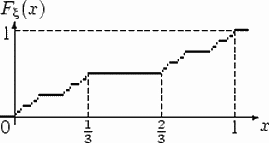
\includegraphics[height=30mm]{kantor}}
\hfill
\parbox[b][3 cm][t]{100mm}{
	Посчитаем меру множества, на котором функция константа, то есть точки этого множества не будут точками роста: сначала это одна ступенька длины 1/3, потом две длины 1/9, и т.д.

}\\
	$$ \frac13 + \frac29 + \frac4{27} = \frac13 \sum\limits_{k=1}^\infty(\frac23)^{k-1} = 1$$
	Тогда множество точек роста имеет меру 0 в силу свойства аддитивности меры.
\end{Ex}
\\

Вообще говоря, существуют менее изысканные примеры сингулярных распределений. Например, при стрельбе из лука в круглую мишень распределение будет сингулярным,
если стрелок попадает только в точки одной прямой. В самом деле, двумерная мера прямой равна 0, как и вероятность попасть в каждую отдельную точку. 

\begin{Th} [Лебега]
	Любую случайную величину можно представить в виде суммы дискретной, абсолютно непрерывной и сингулярной случайной величины. То есть 
	$$ F(x) = \alpha_dF_d(x) + \alpha_cF_c(x) + \alpha_sF_s(x), \quad \alpha_d + \alpha_c + \alpha_s = 1$$
\end{Th}
\begin{Proof}
вышло и не вернулось
\end{Proof}

\newpage
\section{Характеристики случайных величин}

\underline{Математическое ожидание} (обозначается $\Expec$) обобщает понятие среднего арфиметического для произвольной случайной величины и показывает, какие значения в среднем принимает случайная величина. Оно, как и интеграл Лебега, вводится в несколько этапов. В этом определении вероятность $\Pro$ играет роль
Лебеговой меры $\mu$.

\begin{itemize}
 	\item Если $\xi(\omega) = \sum\limits_{i=1}^kx_i \Ind(A_i) \quad (i \not= j \Rightarrow A_iA_j = \varnothing, \ \bigcup_{i=1}^k = \Omega)$. 
 	$$\Expec \xi = \int\limits_{\Omega} \xi(\omega) \Pro(d\omega) \equiv \sum\limits_{i=1}^k x_i \Pro(\Set{\omega}{\xi(\omega)=x_i}) =  \sum\limits_{i=1}^k x_i \Pro(A_i)$$
	\item $\xi(\omega) \ge 0$. В этом случае аналогично интегралу Лебега
	$$ \Expec \xi = \int\limits_{\Omega} \xi d\Pro = \lim_{n \to \infty}  \biggl[  \sum\limits_{k=1}^{n2^n} \frac{k-1}{2^n} \Pro\biggl(\Set{\omega}{\frac{k-1}{2^n} \le \xi(\omega) < \frac{k}{2^n}}\biggl) 
	+ n \Pro(\Set{\omega}{\xi(\omega) \ge n})\biggl]$$
	\item Для произвольной $\xi(\omega)$ вводятся
	$$ \xi^+(\omega) = \max\{0, \xi(\omega)\},\quad \xi^-(\omega) = -\min\{0, \xi(\omega)\}$$
	$$ \Expec \xi = \Expec \xi^+ - \Expec \xi^-$$
\end{itemize}

Вспомним, что любая случайная величина $\xi$ индуцирует вероятностное пространство $(\Real, \Bor_\xi, \Pro_\xi)$. Тогда, поскольку $\Pro_\xi(dx)$ есть вероятность попасть
в $dx$, выразим ее через функцию распределения $\Pro_\xi(dx) = F_\xi(x + dx) - F_\xi(x) = dF_\xi(x)$ Тогда перепишем матожидание в более привычной форме
$$\Expec\xi = \int\limits_{\Omega} \xi(\omega) \Pro(d\omega) = \int\limits_{-\infty}^{+\infty} x \Pro_\xi(dx) = \int\limits_{-\infty}^{+\infty} x dF_\xi(x)$$

Перечислим некоторые свойства математического ожидания:
\begin{enumerate}
	\item $\Expec(\xi + a) = \Expec\xi + a \quad \forall a \in \Real$
	\item $\Expec(a\xi) = a\Expec\xi \quad \forall a \in \Real$
	\item $\Expec(\xi + \eta) = \Expec\xi + \Expec\eta$ (здесь подразумевается, что существуют два из трех математических ожидания, из чего следует существование третьего)
\end{enumerate}
\begin{Ex}
Рассмотрим дискретную случайную величину $\xi$, которая принимает значения $n$ с вероятностью $\frac{c}{n^2} \ (c = \frac{6}{\pi^2})$. По определению
$$ \Expec\xi = \sum\limits_{n=1}^{\infty} n \frac{c}{n^2} $$
Данный ряд, очевидно, расходится. Сиутацию не спасет даже рассмотрение случайной величины $\eta$, принимающей значения $\pm n$ с вероятностью $\frac{c}{2n^2}$, 
которая имеет среднее значение 0, 
поскольку $\Expec\eta = \sum\limits_{n=1}^{\infty} \frac{c}{2n} - \sum\limits_{n=1}^{\infty} \frac{c}{2n}$, что не определено, поскольку интегралы Лебега от $\eta^+$ и $\eta^-$ расходятся.\\
\end{Ex}
\begin{Ex}
Другим примером является распределение Коши с плотностью $p_\xi(x) = \frac{1}{\pi(1+x^2)}$. График этой функции симметричен относительно 0 и похож на горку, из чего
методом пристального взгляда можно сделать вывод, что средним значением должно быть 0. Однако  $
\int\limits_{-\infty}^{+\infty} x dF_\xi(x) =  \int\limits_{-\infty}^{+\infty} x p_\xi(x)dx$ расходится, поэтому математического ожидания не существует.
\end{Ex}

\begin{Def}
\underline{Квантилью} случайной величины $\xi$ порядка $q$ называется величина $l_\xi(q)$:
\[
   	l_\xi(q) \colon 
  	\begin{cases}
  		\Pro(\xi \le l_\xi(q)) \ge q \\
  		\Pro(\xi \ge l_\xi(q) \ge 1-q
  	\end{cases}
  \]
  
  В случае $q=\frac12$ квантиль называется \underline{медианой} и обозначается $\Med\xi$.
  
  Если $q=\frac14$, то $l_\xi$ называется \underline{квартилью}, если $q=\frac1{10}$, \underline{децилью}, а если $q=\frac{1}{100}$ --- \underline{перцентилью}.
\end{Def}

Жизненный смысл медианы заключается в том, что она является точкой, вероятность попасть левее которой равна пероятности попасть правее нее. Аналогично можно 
сказать про квантиль любого порядка. Квантиль определена не единственным образом: пусть $\xi$ принимает значения $\{0, 1\}$ с вероятностями $\frac12$. Тогда медианой
$\xi$ может быть любая точка из отрезка $[0,1]$.

С матожиданием и мединой связана задача о <<деловых людях>>. (здесь будет ссылка) 
\newpage

\section{Виды сходимости случайных величин}

В этом разделе мы введем вагон непонятных определений, а потом постараемся запутаться еще больше, доказывая, какая сходимость круче, и ковыряясь в контрипримерах. Но для начала вспомним наших старых знакомых: измеримое пространство $(\Omega, \Ev)$, вероятностное пространство $(\Omega, \Ev, \Pro)$ и случайную величину $\xi \colon \Omega \rightarrow \Real$, которая обладает свойством
$$\forall B \in \Bor \quad \xi^{-1}(B) = \{ \omega \in \Omega \colon \xi(\omega) \in B \} \in \Ev$$

Пусть теперь $\xi, \xi_1, \xi_2, \dots$ "--- случайные величины на $(\Omega, \Ev)$.

\begin{Def}
Последовательность случайных величин $\{\xi_n\}$ \uline{сходится} к случайной величине $\xi$ \uline{почти наверное (с вероятностью 1)}, если вероятность множества тех элементарных событий, где она не сходится, равно нулю.
$$\{ \xi_n \} \xrightarrow{\text{п.н.}} \xi, \text{если} \quad \Pro(\Set{\omega}{\xi_n(\omega) \nrightarrow \xi}) = 0$$
\end{Def}

\begin{Ex}
Пусть $\xi_n$ принимает значение $n$ в рациональных точках числовой прямой и $0$ "--- в иррациональных. Тогда $\{\xi_n\} \xrightarrow{\text{п.н.}} 0$, так как мера множества рациональных чисел, где случайная величина расходится, "--- ноль.
\end{Ex}

\begin{Def}
Последовательность случайных величин $\{\xi_n\}$ \uline{сходится} к случайной величине $\xi$ \uline{в среднем порядка $r$}, если $r$-тый момент их разности сходится к нулю.
$$\{ \xi_n \} \xrightarrow{\text{(r)}} \xi, \text{если} \quad \Expec(\xi_n - \xi)^r \xrightarrow[n \rightarrow +\infty]{} 0$$
\end{Def}

\begin{Ex}
Возьмем в качестве множества $\Omega$ окружность длины 1, событиями будут борелевские множества, а вероятность введем как меру Лебега. События $A_n$ введем таким образом: $A_1$~"--- дуга длины $1/2$, отложенная от какой-то точки против часовой стрелки. $A_n$~"--- дуга длины $\frac{1}{n+1}$, отложенная против часовой стрелки от конца дуги $A_{n-1}$. Введем случайную величину: $\xi_n(\omega) = \Ind(\omega \in A_n)$
Покажем, что $\{\xi_n\}$ сходится к $0$ в среднем любого положительного порядка.
$$\Expec(\xi_n - \xi)^r = \Expec\xi_n^r = \Expec\left(\Ind(\omega \in A_n)\right)^r = \Pro(A_n) = 1/n \xrightarrow[n \rightarrow +\infty]{} 0$$
\end{Ex}

\begin{St}
Из сходимости в среднем, вообще говоря, не следует сходимость почти наверное.
\end{St}

\begin{Proof}
В рассмотренном выше примере $\xi_n(\omega)$ не сходится ни в одной точке окружности. Действительно, так как ряд $\sum_{n=1}^\infty \frac{1}{n}$ расходится, то для любой точки $\omega$ на окружности мы можем указать бесконечное число номеров $n_k$, таких что $\omega~\in~A_{n_k}$.~
\end{Proof}

\begin{St}
Из сходимости почти наверное, вообще говоря, не следует сходимость в среднем.
\end{St}

\begin{Proof}
Рассмотрим отрезок $[0, 1]$, с событиями, являющимися борелевскими множествами и вероятностью, введенной как мера Лебега. Положим $\xi_n(\omega) = e^{n} \Ind(\omega \in [0, 1/n])$. Тогда $\xi_n \xrightarrow{\text{п.н.}} 0$, но при этом $\forall r > 0 \quad \Expec\xi_n^r = e^{np}\Expec\Ind(\omega \in [0, 1/n]) = e^{np}/n$, а эта величина стремится к бесконечности, значит, сходимости в среднем нет.~
\end{Proof}

Введем еще один вид сходимости.

\begin{Def}
Последовательность случайных величин $\{\xi_n\}$ \uline{сходится} к случайной величине $\xi$ \uline{по вероятности}, если для любого сколь угодно малого положительного $\varepsilon$ вероятность таких событий, что модуль разности $\xi_n$ и $\xi$ больше $\varepsilon$, стремится к $0$.
$$\{\xi_n\} \xrightarrow{\Pro} \xi, \text{если} \quad \forall \varepsilon > 0 \quad \Pro(\Set{\omega}{|\xi_n(\omega) - \xi(\omega)| > \varepsilon}) \xrightarrow[n \rightarrow +\infty]{} 0$$
\end{Def}

\begin{Wtf}
На этом моменте может немного поплавиться мозг в попытках понять, чем сходимость по вероятности отличается от сходимости с вероятностью 1. Действительно, и там и там мы говорим, что вероятность тех событий, на которых случайная величина не сходится, равна нулю. Но разница в том, что в случае сходимости почти наверное мы сначала устремляем $n$ к бесконечности, а потом считаем вероятность, событий, когда не сходится, а в случае сходимости по вероятности мы сначала посчитали вероятность для какого-то фиксированного $n$, а потом устремились к бесконечности. 
\end{Wtf}

\begin{Ex}
Докажем, что та жуткая последовательность случайных величин на окружности сходится по вероятности к нулю. Действительно, 
$$\Pro(\Set{\omega}{|\xi_n(\omega) - 0| > \varepsilon}) = \Pro(\Set{\omega}{\xi_n(\omega) > \varepsilon}) = \Pro(\Set{\omega}{\xi_n(\omega) = 1}) = 1/n \xrightarrow[n \rightarrow +\infty]{} 0$$
\end{Ex}

\begin{St}
Только что рассмотренным примером мы доказали, что из сходимости по вероятности, вообще говоря, не следует сходимость почти наверное.
\end{St}

\begin{St}
Из сходимости по вероятности, вообще говоря, не следует сходимость в среднем.
\end{St}

\begin{Proof}
Для доказательства воспользуемся примером про отрезок. Докажем, что $\{\xi_n\} \xrightarrow{\Pro} 0$. Действительно, $\Pro{\Set{\omega}{\xi_n(\omega) > \varepsilon}} = 1/n \xrightarrow[n \rightarrow +\infty]{} 0$. Отсутствие сходимости в среднем мы уже доказали.
\end{Proof}

\begin{Th}
Из сходимости почти наверное следует сходимость по вероятности.
\end{Th}

\begin{Proof}
Сначала докажем, что $\{ \xi_n \} \xrightarrow{\text{п.н.}} \xi \quad \Leftrightarrow \quad \Pro\left(\sup \limits_{k \geqslant n} |\xi_k -\xi| \geqslant \varepsilon\right) \rightarrow 0$. Положим $A_n^\varepsilon = \Set{\omega}{|\xi_n -\xi| \geqslant \varepsilon}$, 
$A^\varepsilon = \varlimsup A_n^\varepsilon \equiv \bigcap\limits_{n=1}^\infty \bigcup\limits_{k \geqslant n} A_k^\varepsilon$. Тогда:
$$\Pro\left(\Set{\omega}{\xi_n(\omega) \nrightarrow \xi}\right) = 0 \quad \Leftrightarrow \quad \Pro\left(\bigcup_{\varepsilon > 0} A^\varepsilon\right) = 0 \quad \Leftrightarrow \quad \Pro\left(\bigcup_{m=1} A^{1/m}\right) = 0 \quad \Leftrightarrow$$
$$\Leftrightarrow \quad \Pro(A^{1/m}) = 0, m \geqslant 1 \quad \Leftrightarrow \quad \Pro(A^\varepsilon) = 0, \varepsilon > 0 \quad \Leftrightarrow \quad 
\Pro\left( \bigcup_{k \geqslant n} A_k^\varepsilon \right) \xrightarrow[n \rightarrow \infty]{} 0, \varepsilon > 0 \quad \Leftrightarrow$$
$$\Leftrightarrow \quad \Pro\left(\sup \limits_{k \geqslant n} |\xi_k -\xi| \geqslant \varepsilon\right) \xrightarrow[n \rightarrow \infty]{} 0 \quad \Rightarrow \quad \Pro\left( |\xi_k - \xi| \geqslant \varepsilon \right) \rightarrow 0.$$
А последнее утверждение "--- это определение сходимости по вероятности.
\end{Proof}

\begin{Wtf}
Совершенно жуткое доказательство, понимается методом вглядывания: если достаточно долго медитировать над каждой импликацией, то все переходы в конце концов станут понятными.
\end{Wtf}

\begin{Th}
Из сходимости в среднем следует сходимость по вероятности.
\end{Th}

\begin{Proof}
Утвеждение теоремы практически сразу же следует из обобщенного неравентва Чебышева:
$$\Pro \left( |\xi_n - \xi| \geqslant \varepsilon \right) \leqslant \frac{\Expec|\xi_n - \xi|^r}{\varepsilon^r}.$$
Переходя в неравенстве к пределу при $n \rightarrow \infty$, получаем требуемое.
\end{Proof}

\begin{Def}
Последовательность случайных величин $\{\xi_n\}$ \uline{слабо сходится} к случайной величине $\xi$, если для любой непрерывной и ограниченной функии последовательность мат. ожиданий функций от $\xi_n$ сходится к мат. ожиданию функции от $\xi$.
$$\{ \xi_n \} \xrightarrow{w} \xi, \text{если} \quad \forall f(x) \colon f(x) \in C \  \text{и} \  |f(x)| \leqslant M \quad \Expec{f(\xi_n)} \rightarrow \Expec{f(\xi)}$$
\end{Def}

\begin{St}
Из сходимости по вероятности следует слабая сходимость.
\end{St}

\begin{Proof}
Пусть $f(x) \colon |f(x)| \leqslant M.$ Также $\forall \varepsilon > 0$ выберем $N$ так, чтобы $\Pro{|\xi| > N} \leqslant \dfrac{\varepsilon}{4M}.$ Выберем $\delta$ так, чтобы $\forall |x| \leqslant N$ и $|x - y| \leqslant \delta$ было выполнено неравенство $|f(x) - f(y)| \leqslant \varepsilon/2$. Тогда:
\begin{multline*}
	\Expec{|f(\xi_n) - f(\xi)|} =
	\Expec{\left(|f(\xi_n) - f(\xi)|; |\xi_n - \xi| \leqslant \delta; |\xi| \leqslant N\right)} + \\
	\Expec{ \left( |f(\xi_n) - f(\xi)|; |\xi_n - \xi| \leqslant \delta; |\xi| > N \right) } +
	\Expec{ \left( |f(\xi_n) - f(\xi)|; |\xi_n - \xi| > \delta) \right) } \leqslant \\
	\varepsilon/2 + \varepsilon/2 + 2M * \Pro(|\xi_n - \xi| > \delta) = \varepsilon + \Pro(|\xi_n - \xi| > \delta).
\end{multline*}
Но из сходимости по веротности следует, что $\Pro(|\xi_n - \xi| > \delta) \rightarrow 0$, значит при $n~\rightarrow~\infty \qquad \Pro(|\xi_n - \xi| > \delta) < \varepsilon$, тогда $\Expec{|f(\xi_n) - f(\xi)|} < 2\varepsilon$, откуда в силу произвольного выбора $\varepsilon$ и в силу того, что модуль числа не превосходит самого числа, получаем требуемое.
\end{Proof}


\begin{Def}
Последовательность слeчайных величин $\{\xi_n\}$ \uline{сходится} к случайной величине $\xi$ \uline{по распределению}, если функции распределения $\{\xi_n\}$ сходятся к функции распределения $\xi$ во всех точках, в которых предельная функция распределения непрерывна.
$$\{ \xi_n \} \xrightarrow{d} \xi, \text{если} \quad F_{\xi_n}(x) \rightarrow F_\xi \quad \forall x \colon F_\xi(x) \in C(x)$$
\end{Def}

\begin{Ex}
Пусть $\{ \xi_n \}$ принимает значения $0$ и $1 - \dfrac{1}{n}$ с вероятностями $\dfrac{1}{2}$. Тогда функция распределения для случайной величины $\xi_i$ выглядит так (Рис.~\ref{ris:distr_seq}): 
\\
\begin{minipage}{0.32\linewidth}
	\begin{tikzpicture}
	\begin{axis}[
		scale=0.5,
		axis x line = middle,
		axis y line = middle,
		xlabel = {$x$},
		ylabel = {$F_{\xi_n}$},
		domain=-0.2:1.2
		ymin=-0.2,
		ymax=1.2,
		extra x ticks={0.75},
		extra x tick style={
			grid=major
		},
		extra x tick label={$\frac{3}{4}$}
	]
	\addplot[blue, domain=-0.2:0] {0};
	\addplot[blue, mark=*] coordinates {(0, 0)};
	\addplot[blue, mark=o] coordinates {
		(0, 0.5)
		(0.75, 0.5)
	};
	\addplot[blue, mark=*] coordinates {(0.75, 0.5)};
	\addplot[blue, mark=none, domain=0.75:1.2] {1};
	\addplot[blue, mark=o] coordinates {(0.75, 1)};
	\end{axis}
	\end{tikzpicture}
	\captionof{figure}{Функция распределения $\xi_n$ при $n = 4$}
	\label{ris:distr_seq}
\end{minipage}
\hfill
\begin{minipage}{0.32\linewidth}
	\begin{tikzpicture}
	\begin{axis}[
		scale=0.5,
		axis x line = middle,
		axis y line = middle,
		xlabel = {$x$},
		ylabel = {$F_{\xi_n}$},
		domain=-0.2:1.2
		ymin=-0.2,
		ymax=1.2
	]
	\addplot[blue, domain=-0.2:0] {0};
	\addplot[blue, mark=*] coordinates {(0, 0)};
	\addplot[blue, mark=o] coordinates {
		(0, 0.5)
		(1, 0.5)
	};
	\addplot[blue, mark=none, domain=1:1.2] {1};
	\addplot[blue, mark=*] coordinates {(1, 1)};
	\end{axis}
	\end{tikzpicture}
	\captionof{figure}{Предельная функция}
	\label{ris:limit_f}
\end{minipage}
\hfill
\begin{minipage}{0.32\linewidth}
	\begin{tikzpicture}
	\begin{axis}[
		scale=0.5,
		axis x line = middle,
		axis y line = middle,
		xlabel = {$x$},
		ylabel = {$F_{\xi_n}$},
		domain=-0.2:1.2
		ymin=-0.2,
		ymax=1.2
	]
	\addplot[blue, domain=-0.2:0] {0};
	\addplot[blue, mark=*] coordinates {(0, 0)};
	\addplot[blue, mark=o] coordinates {
		(0, 0.5)
		(1, 0.5)
	};
	\addplot[blue, mark=*] coordinates {(1, 0.5)};
	\addplot[blue, mark=none, domain=1:1.2] {1};
	\addplot[blue, mark=o] coordinates {(1, 1)};
	\end{axis}
\end{tikzpicture}
\captionof{figure}{Функция распределения $\xi$}
\label{ris:dist_lim}
\end{minipage}
\par\bigskip
Тогда предельная функция будет выглядеть так (Рис.~\ref{ris:limit_f}). Заметим, что она вообще не является функцией распределения, так как в точке $1$ нарушено условие непрерывности слева. Тогда рассмотрим случайную величину $\xi$, принимающую значение $0$ и $1$ с вероятностями $1/2$, тогда ее функция распределения имеет вид (Рис.~\ref{ris:dist_lim}). Заметим, что предельная функция и функция распределения $\xi$ различаются только в точке $1$, в которой $F_\xi(x)$ не является непрерывной, значит $\{\xi_n\} \xrightarrow[]{d} \xi.$
\end{Ex}

\begin{St}
Сходимость по распределению эквивалентна слабой сходимости.
\end{St}

\begin{Proof}
\uline{\textbf{TODO:}} Чет я не знаю, как это доказать =(
\end{Proof}

\begin{St}
Если последовательность случайных величин $\{ \xi_n \}$ сходится по распределению к вырожденной случайной величине $\xi \xequiv{\text{п.н.}} a$, то $\{ \xi_n \}$ сходится к $\xi$ по вероятности.
\end{St}

\begin{Proof}
Ы
\end{Proof}

А теперь докажем теорему, ради которой мы и городили все эти огороды сходимостей. Эта теорема впоследствии будет использоваться при доказательстве центральной предельной теоремы.

\begin{Th}[теорема Леви о непрерывности]
~\\
\begin{enumerate}
	\item Пусть $\{ \xi_n \} \xrightarrow{d} \xi$ \ и \ $f_n(t) := \Expec e^{it\xi_n}$.\ Тогда $\{ f_n(t) \} \rightarrow f(t)$,\ где $f(t) = \Expec e^{it\xi}$.
	\item Пусть теперь $f_n(t) := \Expec e^{it\xi_n}$. Тогда если $f_n(t) \rightarrow f(t) \quad \forall t \in \Real, \quad f(t) \in C(0)$, то $f(t)$ является характеристической функцией некоторой случайной величины $\xi$, такой что $\{ \xi_n \} \xrightarrow{d} \xi.$ 
\end{enumerate}
\end{Th}

\begin{Proof}
\begin{enumerate}
	\item Как было показано выше, сходимость по распределению эквивалентна слабой сходимости. Положим в определении слабой сходимость функции $\phi(x) := Re(e^{itx})$ и $\psi(x) := Im(e^{itx})$, тогда $\Expec\phi(\xi_n) \rightarrow \Expec\phi(\xi)$ и $\Expec\psi(\xi_n) \rightarrow \Expec\psi(\xi)$, откуда следует утверждение теоремы.
	\item Достаточно грустное доказательство, но, если у меня будет настроение, я его напишу. 
\end{enumerate}
\end{Proof}

\begin{Wtf}
А вот картинка, на которой схематично показано, что из чего следует.
\end{Wtf}

\begin{center}
\begin{tikzpicture}
	[
		st/.style={rectangle,draw}
	]
	\node[st] (prob1) {$\{ \xi_n \} \xrightarrow{\text{п.н.}} \xi$};
	\node[rectangle] (empty) [below=of prob1] {~};
	\node[st] (power) [below=of empty] {$\{ \xi_n \} \xrightarrow{(r)} \xi$};
	\node[st] (pro) [right=of empty] {$\{ \xi_n \} \xrightarrow{(\Pro)} \xi$};
	\node[st] (distr) [right=of pro] {$\{ \xi_n \} \xrightarrow{(d)} \xi$};
	\node[st] (weak) [below=of distr] {$\{ \xi_n \} \xrightarrow{(w)} \xi$};	
	\node (pn) at (3.8, -0.2) {$\xi \xequiv{\text{п.н.}} a$};
	\node[st] (th) [right=of distr] {т. о непрерывности};
	
	\draw [->] (prob1) -> (pro);
	\draw [->] (power) -> (pro);
	\draw [->] (pro) -> (distr);
	\draw [<->] (distr) -> (weak);
	\draw [->] (distr) to[bend right=45] (pro);
	\draw [dotted, line width=2pt] (distr) -> (th);
\end{tikzpicture}
\end{center}


\end{document}